\documentclass[aps,pra,twocolumn,superscriptaddress,floatfix,nofootinbib]{revtex4-2}
\usepackage{amsmath,amssymb,amsthm,mathtools}
\usepackage{graphicx}
\usepackage{tikz}
\usetikzlibrary{arrows.meta,positioning,calc,decorations.markings,shapes.geometric}
\usepackage[colorlinks=true,linkcolor=blue!50!black,citecolor=blue!50!black,urlcolor=blue!50!black]{hyperref}

\newtheorem{theorem}{Theorem}
\newtheorem{proposition}[theorem]{Proposition}
\newtheorem{lemma}[theorem]{Lemma}
\newtheorem{corollary}[theorem]{Corollary}
\theoremstyle{definition}
\newtheorem{definition}{Definition}
\newtheorem{example}{Example}

\newcommand{\NN}{\mathcal N_1}
\newcommand{\D}{\mathbb D}
\newcommand{\one}{\mathbf 1}
\newcommand{\T}{\mathsf T}
\newcommand{\Cost}{\mathrm{Cost}}

\begin{document}

\title{Non-reciprocity as a resource: budget and noise bounds,\\ and what the non-Hermitian skin effect buys}

\author{Marcelo Group}
\date{Draft, October 16, 2026}

\begin{abstract}
Non-reciprocity is widely described as a resource for classical and quantum technologies. We formulate a resource theory of Lorentz non-reciprocity for linear networks, in which the free objects are Lorentz-reciprocal and the free operations embed an object into an arbitrary reciprocal network, with loops, resonances and interference allowed. For passive networks we prove that the bandwidth-averaged non-reciprocity is bounded by the sum of the non-reciprocities of the elementary components. For two-ports this is an isolation--bandwidth bound. The bound is tight but is not itself a monotone; the monotone is the elementary cost. With reciprocal gain the classical theory collapses, since one loop and one amplifier turn any weak element into a perfect directional amplifier. Two structures survive. In loop-free networks the imaginary gauge flux is exactly conserved, even with gain. With loops, non-reciprocity beyond the budget costs quantum noise at the non-reciprocal elements, by a tight inequality. For lattices, robust stability requires $|S_{21}/S_{12}|>r^2G$, so a series amplifier chain can be stable at all lengths only if its gain rate does not exceed its gauge-flux rate: extensive stable gain needs the Hatano--Nelson skin effect. Finally, a network winding number vanishes for passive cells, for reciprocal cells and for single-channel phase-only cells. A driven skin effect therefore needs gain and non-reciprocity, and phase-only non-reciprocity needs a loop.
\end{abstract}

\maketitle

%======================================================================
\section{Introduction}

Isolators, circulators and directional amplifiers route signals one way, and they are indispensable wherever a fragile source must be protected from its own readout chain \cite{Jal13,Cal18,Bar25}. A recent review calls non-reciprocity ``a powerful resource in quantum technologies'' \cite{Bar25}. Resource theories \cite{CG19} of related symmetries exist: for PT-type antiunitary asymmetry of states \cite{BFPW16} and, very recently, a dynamical resource theory of time-reversal-symmetry breaking for quantum channels \cite{MKM26}. They work with antiunitary symmetries of states and channels. A device designer needs something different: Lorentz reciprocity, $S=S^\T$ for a multiport scattering response, which differs from time-reversal symmetry once loss or gain is present \cite{Jal13,Cal18}; objects that are dispersive, so that bandwidth matters; composition by networks with loops and resonances; and an account of gain and amplifier noise. For this setting we are not aware of a specification of what can be done for free, of a monotone that free operations cannot increase, or of an accounting of what a given amount of non-reciprocity can buy.

A related development is the non-Hermitian skin effect (NHSE): under open boundaries an extensive number of eigenmodes of a non-Hermitian lattice accumulate at a boundary \cite{HN96,YW18,KEBB18,AGU20,BBK21}. In one dimension the NHSE is equivalent to a non-zero point-gap winding \cite{OKSS20,ZYF20}, and it can be read off from the transfer matrix \cite{KD19}. It underlies exponentially large directional amplification \cite{Por19,WBN20,WBN21,ZRR21,Xue21,BWN23} and sensing \cite{MC20}. It is natural to ask whether the skin effect is itself a resource. We argue that the useful resource is non-reciprocity. The skin effect is what that resource looks like in an extended system, and we identify precisely what it buys.

\begin{figure*}[t]
\centering
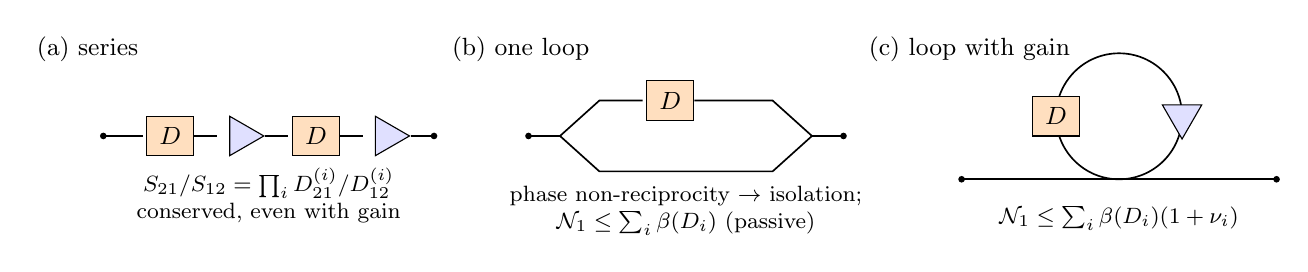
\begin{tikzpicture}[>=Stealth, font=\small,
  dev/.style={draw, fill=orange!25, minimum width=6mm, minimum height=5mm, inner sep=1pt},
  amp/.style={draw, isosceles triangle, isosceles triangle apex angle=60, fill=blue!12, minimum width=5mm, inner sep=0pt},
  wire/.style={line width=0.6pt}]
% (a) series
\begin{scope}
\node at (-0.2,1.1) {(a) series};
\draw[wire] (0,0) -- (0.5,0);
\node[dev] (d1) at (0.85,0) {$D$};
\draw[wire] (d1.east) -- (1.45,0);
\node[amp] (a1) at (1.75,0) {};
\draw[wire] (a1.east) -- (2.35,0);
\node[dev] (d2) at (2.7,0) {$D$};
\draw[wire] (d2.east) -- (3.3,0);
\node[amp] (a2) at (3.6,0) {};
\draw[wire] (a2.east) -- (4.2,0);
\fill (0,0) circle (1.2pt); \fill (4.2,0) circle (1.2pt);
\node[align=center, font=\footnotesize] at (2.1,-0.75) {$S_{21}/S_{12}=\prod_i D^{(i)}_{21}/D^{(i)}_{12}$\\ conserved, even with gain};
\end{scope}
% (b) MZI loop
\begin{scope}[xshift=5.4cm]
\node at (-0.1,1.1) {(b) one loop};
\draw[wire] (0,0) -- (0.4,0);
\draw[wire] (0.4,0) -- (0.9,0.45) -- (1.45,0.45);
\draw[wire] (0.4,0) -- (0.9,-0.45) -- (3.1,-0.45) -- (3.6,0);
\node[dev] (d3) at (1.8,0.45) {$D$};
\draw[wire] (d3.east) -- (3.1,0.45) -- (3.6,0) -- (4.0,0);
\fill (0,0) circle (1.2pt); \fill (4.0,0) circle (1.2pt);
\node[align=center, font=\footnotesize] at (2.0,-0.95) {phase non-reciprocity $\to$ isolation;\\ $\NN\le\sum_i\beta(D_i)$ (passive)};
\end{scope}
% (c) loop with gain
\begin{scope}[xshift=10.9cm]
\node at (0.1,1.1) {(c) loop with gain};
\draw[wire] (0,-0.55) -- (4.0,-0.55);
\draw[wire] (2.0,0.25) circle (0.8);
\node[dev] at (1.2,0.25) {$D$};
\node[amp, rotate=-90] at (2.8,0.25) {};
\fill (0,-0.55) circle (1.2pt); \fill (4.0,-0.55) circle (1.2pt);
\node[align=center, font=\footnotesize] at (2.0,-1.05) {$\NN\le\sum_i\beta(D_i)(1+\nu_i)$};
\end{scope}
\end{tikzpicture}
\caption{The three geometries that organize the results. (a) In a series (loop-free) network the ratio $S_{21}/S_{12}$, the imaginary gauge flux, is a product of local ratios and is unaffected by reciprocal gain or loss (Proposition~\ref{prop:series}). (b) A loop converts phase-type non-reciprocity into directionality; without gain the bandwidth-averaged non-reciprocity $\NN$ is bounded by the elementary budget (Theorem~\ref{thm:budget}). (c) With gain inside a loop, $\NN$ can exceed the budget, but only by exposing the elements to amplifier noise (Theorem~\ref{thm:noise}).}
\label{fig:geometries}
\end{figure*}

We take the free operations to be those that Lorentz reciprocity allows. Linear, time-invariant components without magnetic or other time-odd bias are reciprocal, and so are networks built from them \cite{Jal13,Cal18}. ``One cannot build an isolator from reciprocal parts'' is then the analogue of ``one cannot create entanglement by local operations and classical communication''. In this setting, objects are linear networks seen from their ports. Free operations insert an object once into an arbitrary reciprocal network, and the resource enters through elementary non-reciprocal devices. Our main results are the following:
\begin{enumerate}
\item A \emph{budget theorem} for passive networks: the bandwidth-averaged non-reciprocity is bounded by the sum of the elementary non-reciprocities, tightly, whatever loops, resonances or interferometers are used (Theorem~\ref{thm:budget}). It implies an isolation--bandwidth bound. The bound is not a monotone on dispersive objects, and closing a narrowband isolator into a loop more than doubles it. The monotone is the elementary cost (Proposition~\ref{prop:cost}).
\item A \emph{loop principle}. In series networks $S_{21}/S_{12}$ is exactly multiplicative, so pure-phase elements never isolate. A single loop turns $\pi/\Delta$ of them into a perfect broadband isolator. The lattice analogue is that nearest-neighbour chains with $|t^+|=|t^-|$ are reciprocal up to gauge, while chains with loops show a skin effect driven by phases alone.
\item \emph{Gain}. With free reciprocal gain the classical theory collapses (Theorem~\ref{thm:collapse}). In series networks the gauge flux remains exactly conserved and is a complete invariant at fixed frequency. With loops, a tight \emph{noise-price} inequality holds: $\NN\le\sum_i\beta(D_i)(1+\nu_i)$, where $\nu_i$ counts the amplifier noise quanta that reach element $i$ (Theorem~\ref{thm:noise}).
\item \emph{What the skin effect buys}. A robustly stable amplifier needs $|S_{21}/S_{12}|>r^2G$, so a series chain is stable at every length only if its gain rate does not exceed its gauge-flux rate (Theorem~\ref{thm:stab}). A network winding number vanishes for passive, for reciprocal and for single-channel phase-only cells (Theorem~\ref{thm:winding}).
\end{enumerate}
Several ingredients and qualitative statements are known, and we state them precisely here. The transfer-matrix determinant is classical (a reciprocal two-port has $AD-BC=1$ \cite{Poz12}), as are the symplectic structure of reciprocal transfer matrices and the unconditional-stability condition \cite{Rol62}. That non-reciprocity in coupled-mode systems requires a loop threaded by a non-trivial phase is known \cite{RA15,MC15}. The transfer-matrix criterion for the skin effect \cite{KD19}, the correspondence between winding and directional amplification \cite{Por19,WBN20,WBN21,BWN23}, and the instability of open-boundary directional amplifiers when the boundary is closed \cite{WBN20,Xue21} are also known. So is the fact that non-reciprocal amplification can be quantum limited \cite{Kam11,MC15,Mal18}. Classical network synthesis asks how many gyrators a given non-reciprocal immittance requires \cite{AV73}, and time--bandwidth limits of non-reciprocal cavities have been analysed \cite{MSA19}. To our knowledge, the budget and noise-price bounds (Theorems~\ref{thm:budget} and~\ref{thm:noise}) and the cost monotone are new. Theorems~\ref{thm:stab} and~\ref{thm:winding} recast and sharpen known correspondences in the language of scattering networks, where they become statements about the resource. Skin effects of reciprocal origin, such as the geometry-dependent skin effect of two-dimensional lattices \cite{ZYF22,Wan23} and the $\mathbb Z_2$ skin effect \cite{OKSS20,KSUS19}, are free here. Within the quasi-one-dimensional networks we treat, they can neither isolate nor directionally amplify (Theorem~\ref{thm:winding}). All numerical statements are reproduced by the code described in Appendix~\ref{app:num}.

%======================================================================
\section{Networks and the resource theory}\label{sec:setting}

\begin{definition}[Network]\label{def:net}
A network consists of \emph{junctions} with constant scattering matrices $S_k$, whose ports form a set $P$, with $S_J=\bigoplus_kS_k$. The ports split as $P=E\sqcup I$ into external and internal ports. Internal ports are matched in pairs by \emph{lines} $\ell=\{p,q\}$ with delay $d_\ell\in\{1,2,\dots\}$ and amplitude $|a_\ell|\le1$, the same in both directions, so that the connection matrix $C(z)$, with $C_{pq}=C_{qp}=a_\ell z^{d_\ell}$, is symmetric. The response is
\begin{equation}
S(z)=S_{EE}+S_{EI}\,C(z)\bigl(\one-S_{II}C(z)\bigr)^{-1}S_{IE}.
\label{eq:response}
\end{equation}
A junction is \emph{reciprocal} if $S_k=S_k^\T$, and \emph{passive} if $\|S_k\|\le1$. A non-reciprocal passive junction is a \emph{device}, and its \emph{budget} is $\beta(D)=\tfrac12\|D_A\|_1$ with $D_A=\tfrac12(D-D^\T)$.
\end{definition}

Here $z^d$ is a delay of $d$ time steps, and $z=e^{i\varphi}$ on the unit circle, with $\varphi$ the frequency in units of the inverse unit delay. The same matrices describe classical waves and, for passive networks, the mode operators of linear quantum optics. For passive networks, $\|S_{II}C(z)\|\le|z|$, so $S$ is analytic and contractive on the unit disk $\D$ and has boundary values almost everywhere \cite{Gar07}. If all junctions are reciprocal, then $S^\T=S$, by the push-through identity $C(\one-S_{II}C)^{-1}=(\one-CS_{II})^{-1}C$.

\begin{definition}[Resource theory]
An \emph{object} is the response of a network, and it is \emph{free} if $S^\T=S$. A \emph{free operation} $\Theta$ inserts an object once into a network all of whose junctions are reciprocal (and, until Sec.~\ref{sec:gain}, passive). The object's ports are joined to that network by lines, and $\Theta(S)$ is the composite response, a Redheffer star product \cite{Red60}.
\end{definition}

Free operations map free objects to free objects. Loops, resonances and interference are all allowed. The budget $\beta$ of a two-port device $D=\left(\begin{smallmatrix}0&D_{12}\\D_{21}&0\end{smallmatrix}\right)$ is $\frac12|D_{21}-D_{12}|$. It equals $\sin\frac\Delta2$ for a pure-phase element ($|D_{21}|=|D_{12}|=1$, relative phase $\Delta$) and $\frac12$ for a perfect isolator.

%======================================================================
\section{Passive networks}\label{sec:passive}

\subsection{The budget theorem}

Define the bandwidth-averaged non-reciprocity
\begin{equation}
\NN(S)=\int_0^{2\pi}\tfrac12\bigl\|S_A(e^{i\varphi})\bigr\|_1\,\frac{d\varphi}{2\pi},\qquad S_A=\tfrac12(S-S^\T).
\end{equation}

\begin{theorem}[Budget]\label{thm:budget}
Let $S$ be the response of a passive network whose devices are $D_1,\dots,D_m$. Then
\begin{equation}
\NN(S)\le\sum_{i=1}^m\beta(D_i),
\end{equation}
with equality when a single device is wired directly to the external ports.
\end{theorem}

The proof (Appendix~\ref{app:budget}) has three steps. First, with external ports on reciprocal junctions, $S_A(z)=X(z)\,\Delta\,X(z)^\T$, where $\Delta=\bigoplus_iD_{i,A}$ and $X=S_{EI}(\one-CS_{II})^{-1}C$ restricted to the device ports. Second, for every constant vector $s$, $\int|X(e^{i\varphi})s|^2d\varphi/2\pi\le|s|^2$: the left side is the energy that leaves the network after the waves $s$ are launched from the device ports at $t=0$. Third, a Youla decomposition of $\Delta$ into rank-two skew blocks \cite{You61}, together with Cauchy--Schwarz, gives the bound.

\begin{corollary}[Isolation--bandwidth]\label{cor:isoband}
For a two-port built from two-port devices, $\int\bigl||S_{21}|-|S_{12}|\bigr|\frac{d\varphi}{2\pi}\le\sum_i|D^{(i)}_{21}-D^{(i)}_{12}|$. An isolator with $|S_{21}|\ge T$ and $|S_{12}|\le L$ on a fraction $f$ of the band therefore needs at least $f(T-L)/(2\sin\frac\Delta2)$ pure-phase elements, whatever resonators or interferometers are used.
\end{corollary}

Figure~\ref{fig:budget}(a) illustrates the corollary. A critically coupled ring around a weak pure-phase element isolates perfectly at one frequency \cite{Bi11}, and its local non-reciprocity exceeds the element's budget by more than an order of magnitude. The band average, however, stays below the budget, and it shrinks as the quality factor grows.

\begin{figure*}[t]
\centering
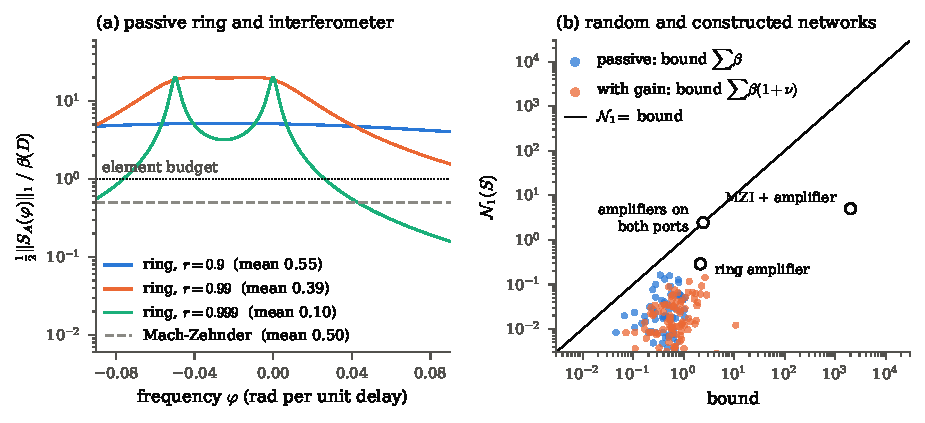
\includegraphics[width=\textwidth]{fig2_budget_noise.pdf}
\caption{(a) Local non-reciprocity $\frac12\|S_A(\varphi)\|_1$, in units of the element budget, for a critically coupled ring around a pure-phase element ($\Delta=0.05$) at three coupling strengths, and for a Mach--Zehnder interferometer containing the same element. Peaks exceed the budget, but band averages (legend) do not (Theorem~\ref{thm:budget}). (b) $\NN$ against its bound for random passive networks (bound $\sum\beta$) and random stable networks with gain (bound $\sum\beta(1+\nu)$), with three constructed examples. Every point lies on or below the diagonal; amplifiers on both ports of a device attain it (Theorem~\ref{thm:noise}).}
\label{fig:budget}
\end{figure*}

\subsection{What is, and is not, a monotone}

\begin{proposition}[Elementary cost]\label{prop:cost}
Let $\Cost(S)$ be the infimum of $\sum_i\beta(D_i)$ over all networks realizing $S$. Then $\Cost(\Theta(S))\le\Cost(S)$ for every free operation $\Theta$, and $\Cost\ge\NN$. Moreover, $\Cost(S)>0$ whenever $S$ is not free.
\end{proposition}

\begin{proof}
A realization of $S$ followed by $\Theta$ is a realization of $\Theta(S)$ with the same devices, and Theorem~\ref{thm:budget} applies to every realization. If $S_A\not\equiv0$, its boundary values cannot vanish on a set of positive measure \cite{Gar07}, so $\NN(S)>0$.
\end{proof}

$\NN$ itself is not a monotone. Take the ring of Fig.~\ref{fig:budget}(a) with $r=0.99$ and a device $0.99\left(\begin{smallmatrix}0&e^{0.05i}\\1&0\end{smallmatrix}\right)$, and close it into a larger loop with one lossless coupler of self-coupling $\frac12$. This raises $\NN$ from $0.00976$ to $0.0213$, a factor of $2.18$ that is converged in quadrature, still below the element budget $0.0247$. A narrowband object leaves part of its budget unused, and a free loop recovers some of it. Consequently $\Cost(R)\ge2.18\,\NN(R)$ for this ring object $R$. Single-frequency quantities fail more badly. In an equal-arm Mach--Zehnder interferometer with a pure-phase element in one arm and a reciprocal amplitude $-e^{i\Delta}(1-\varepsilon)$ in the other, the isolation ratio is frequency-independent and of order $|1-e^{i\Delta}|/\varepsilon$. It is therefore unbounded, even though the element alone has ratio one. Neither the isolation ratio at a frequency nor its band average is a monotone.

\subsection{Loops}

\begin{proposition}[Series networks and transfer matrices]\label{prop:series}
For a $2m$-port with left and right port groups and invertible $S_{12}$, the transfer matrix $T:(a_L,b_L)\mapsto(b_R,a_R)$ satisfies $\det T=\det S_{21}/\det S_{12}$, and cascading multiplies transfer matrices. If $S=S^\T$, with any gain, loss or internal loops, then $T^\T\Omega T=\Omega$ with $\Omega=\left(\begin{smallmatrix}0&\one\\-\one&0\end{smallmatrix}\right)$, so $\det T=1$ and the spectrum of $T$ is closed under $\mu\mapsto1/\mu$. In particular, in a series network of two-ports, $S_{21}/S_{12}=\prod_iS^{(i)}_{21}/S^{(i)}_{12}$ at every frequency.
\end{proposition}

\begin{proof}
For $\det T$, take the Schur complement with respect to the $(2,2)$ block $S_{12}^{-1}$. Reciprocity gives $\sum_p(a_pb'_p-b_pa'_p)=a^\T(S-S^\T)a'=0$ for any two solutions. Split into left and right ports, this is $T^\T\Omega T=\Omega$. A complex symplectic matrix has determinant one, and $T^{-1}=\Omega^{-1}T^\T\Omega$.
\end{proof}

Two consequences follow. Reciprocal parts never change $|S_{21}/S_{12}|$ in series, so pure-phase elements in series never isolate. A single loop suffices to change this. Place $N$ pure-phase elements, with $N\Delta=\pi$, in one arm of a Mach--Zehnder interferometer built from ideal Y-junctions, and a lossless line of equal delay in the other arm. The result has $S_{21}=z^{N+1}$ and $S_{12}=0$ at every frequency, a perfect broadband isolator with $\NN=\frac12$. Its budget $N\sin\frac\Delta2\to\frac\pi2$, so the conversion efficiency is $1/\pi$, against the upper limit $1$ set by Theorem~\ref{thm:budget}.

The lattice analogue is exact. For a tridiagonal $H$ with arbitrary complex diagonal and hoppings $t^\pm_n$, the $(N,1)$ and $(1,N)$ cofactors of $z-H$ are triangular, so $G_{N1}/G_{1N}=\prod_nt^+_n/t^-_n$ for every $z$, with $G=(z-H)^{-1}$. This is the imaginary gauge flux \cite{HN96}. If $|t^+_n|=|t^-_n|$, a diagonal unitary gauge makes $H$ complex symmetric. Then $|G_{mn}|=|G_{nm}|$, and in the translation-invariant case the point-gap winding vanishes. Phase-only non-reciprocity becomes physical only on loops, in agreement with the graph analysis of coupled-mode systems \cite{RA15}. For the chain with $t_{\pm1}=\frac12$, $t_2=-\frac14$, $t_{-2}=+\frac14$ (all magnitudes equal, loop product $t_1^2t_{-2}/t_{-1}^2t_2=-1$), the periodic-boundary curve $h(k)=\cos k+\frac i2\sin2k$ is a figure eight with lobes of winding $-1$ (left) and $+1$ (right). In 60-digit arithmetic up to $N=50$, the end-to-end Green's function grows exponentially in the direction set by the winding.

%======================================================================
\section{Gain and quantum noise}\label{sec:gain}

Now allow reciprocal junctions with $\|S_k\|>1$, such as the amplifier $g\sigma_x$. Lines and devices remain passive. A network is \emph{stable} if $\det(\one-S_{II}C(z))\neq0$ for $|z|\le1$. This determinant is a polynomial equal to $1$ at $z=0$, so stability means that impulse responses decay.

\begin{theorem}[Collapse]\label{thm:collapse}
Let $D=\left(\begin{smallmatrix}0&D_{12}\\D_{21}&0\end{smallmatrix}\right)$ with $D_{21}\neq D_{12}$. Place $D$ in one arm of a Mach--Zehnder interferometer, the reciprocal amplitude $-D_{12}$ in the other arm, and an amplifier $g\sigma_x$ with $g=2\sqrt G/|D_{21}-D_{12}|$ at the output. The result is a stable network with $S_{12}\equiv S_{11}\equiv S_{22}\equiv0$ and $|S_{21}|^2\equiv G$: a perfect broadband directional amplifier of arbitrary gain.
\end{theorem}

The proof is a direct computation, and the signal-flow graph has no directed cycle. If gain is free and noise is not counted, every non-reciprocal device is therefore as good as every other. Two structures nevertheless survive.

\begin{proposition}[Gauge flux with gain]\label{prop:seriesgain}
Proposition~\ref{prop:series} holds with amplifiers, because a reciprocal two-port of any gain has $\det T=1$. In a series network, $\log|S_{21}/S_{12}|$ is therefore exactly conserved and additive. At fixed frequency the ratio is also a complete invariant: if $A$ and $B$ have equal ratios, then $T_BT_A^{-1}$ has determinant one, so (generically) $B$ is $A$ followed by a reciprocal two-port. A series directional amplifier with forward power gain $G$ and backward gain $\le1$ needs $\prod_i|D^{(i)}_{21}/D^{(i)}_{12}|\ge\sqrt G$.
\end{proposition}

With loops, gain must be paid for in noise. Junction $k$ adds noise operators $\xi$ with $[\xi_i,\xi_j^\dagger]=(\one-S_kS_k^\dagger)_{ij}$. The normal-ordered matrix $X_k=(\langle\xi_j^\dagger\xi_i\rangle)$ and the antinormal matrix $X_k+\one-S_kS_k^\dagger$ are both positive semidefinite, so every physical realization has $X_k\ge0$ and $X_k\ge S_kS_k^\dagger-\one$ \cite{Cav82,Cle10}. Let $N_i(\varphi)$ be the spectral matrix of noise quanta arriving at the input ports of device $i$, and let $\nu_i=\lambda_{\max}\int N_i\,d\varphi/2\pi$.

\begin{theorem}[Noise price]\label{thm:noise}
For every stable network with gain, passive devices $D_i$, and every physical noise assignment,
\begin{equation}
\NN(S)\le\sum_i\beta(D_i)\,(1+\nu_i).
\end{equation}
Equality holds for a device with an amplifier $g\sigma_x$ on each of its ports.
\end{theorem}

The proof (Appendix~\ref{app:noise}) replaces the energy argument of Theorem~\ref{thm:budget} by an energy balance that includes the energy gained in the amplifiers. It then shows, by transposing the network, that this gain energy equals the noise arriving at the devices. A weak element's band-averaged effect can be raised by a factor $F$ only if at least $F-1$ quanta per mode reach the element itself. The price is paid at the element and not necessarily at the output. A ring with a lossless coupler ($r=0.9$), an amplifier $1.1105\,\sigma_x$ and a pure-phase element ($\Delta=0.02$) illustrates this. At its peak it has $|S_{21}|^2=1.45\times10^5$ and $|S_{12}|^2=111$, its external added noise exceeds the quantum limit by less than $10^{-9}$ quanta, and $\NN=28.8\,\beta$, which is consistent with $1+\nu=213$. No bound on $\NN$ in terms of the external \emph{excess} noise can therefore hold. This agrees with the existence of quantum-limited directional amplifiers \cite{Kam11,MC15,Mal18}: Theorem~\ref{thm:noise} does not forbid them, but it places the price inside the network. Those devices obtain gain and non-reciprocity from the same parametric coupling, so in our language they are non-passive devices, to which the theorem does not apply. Figure~\ref{fig:budget}(b) tests Theorem~\ref{thm:noise} on random networks.

Gain also changes how the skin effect appears. A chain of $N$ bonds, each with a magnitude element $\left(\begin{smallmatrix}0&e^{-2\gamma}\\1&0\end{smallmatrix}\right)$ ($\gamma=0.15$) and an amplifier $1.15\,\sigma_x$, separated by partial mirrors ($\rho=0.2$), has $|S_{21}/S_{12}|=e^{2\gamma N}$ at every frequency (Proposition~\ref{prop:seriesgain}). Its peak gain is $86$ at $N=16$, and its band-averaged noise approaches the quantum limit (ratio $1.15$). The exponential directionality is the gauge flux; gain only sets the level, and it costs noise.

%======================================================================
\section{Lattices: what the skin effect buys}\label{sec:lattice}

\begin{theorem}[Stable gain needs directionality]\label{thm:stab}
Let $S$ be the response of a stable network with $S_{11}\equiv S_{22}\equiv0$. Terminate its ports through unit lines with constant reflections $|\rho_k|\le r$. The terminated network is stable for every such choice if and only if $r^2|S_{12}S_{21}|<1$ on the unit circle. Hence $G(\varphi)=|S_{21}|^2<r^{-2}|S_{21}/S_{12}|$.
\end{theorem}

\begin{proof}
Termination multiplies the characteristic function by $1-\rho_1\rho_2z^4S_{21}S_{12}$. If $r^2|S_{12}S_{21}|<1$ on the circle, the maximum principle excludes zeros in $|z|\le1$. Otherwise, at a frequency where $r^2|S_{12}S_{21}|\ge1$, a choice of $|\rho_1\rho_2|\le r^2$ and phase puts a zero on the circle. This is the matched case of the unconditional-stability condition \cite{Rol62}.
\end{proof}

\begin{corollary}[Gain rate $\le$ flux rate]\label{cor:rate}
In a series network, $G<r^{-2}\prod_i|D^{(i)}_{21}/D^{(i)}_{12}|$. Consider a chain of $N$ identical matched cells with $|S^{\rm cell}_{21}|=t$ and flux $\lambda=\log|S^{\rm cell}_{21}/S^{\rm cell}_{12}|$, and let $r<1$. It is stable under all terminations $|\rho|\le r$ for every $N$ if and only if $2\log t\le\lambda$ at every frequency.
\end{corollary}

Exponential stable gain thus requires an extensive gauge flux, which is the Hatano--Nelson skin effect. Reciprocal amplifier chains are limited by their Fabry--P\'erot threshold. Figure~\ref{fig:lattice}(a) shows that the same threshold governs chains with internal reflections, which Corollary~\ref{cor:rate} does not cover: long chains are stable only when the gauge flux per bond is at least the log-gain per bond.

\begin{theorem}[Network winding]\label{thm:winding}
For a periodic chain of $m$-channel cells, let $\mu_k(z)$ be the eigenvalues of the cell transfer matrix, assumed not to lie on the unit circle, and define $w(z)=\#\{k:|\mu_k|<1\}-m$. Then $w\equiv0$ if the cell is (i) passive, (ii) reciprocal (with any gain), or (iii) single-channel with $|S^{\rm cell}_{21}/S^{\rm cell}_{12}|=1$.
\end{theorem}

The proof is in Appendix~\ref{app:winding}. Case (i) uses the passivity form $T^\dagger JT\le J$ with $J=\mathrm{diag}(\one,-\one)$. Case (ii) uses the pairing of Proposition~\ref{prop:series}, and case (iii) uses $\mu_1\mu_2=\det T$; it is the scattering counterpart of the transfer-matrix criterion of Ref.~\cite{KD19}. A driven skin effect ($w\ne0$) therefore requires both gain and non-reciprocity. With phase-only non-reciprocity ($|\det T|=1$) it also requires at least two channels, that is, a loop. Random two-channel phase-only cells with gain do show $w\neq0$ (39 of 1000), whereas no passive, reciprocal or single-channel phase-only cell does. In the chain above, $w=-1$ on $91\%$ of the band. There the end-to-end forward gain grows at the rate $\log|\mu_1|$, and it decays where $w=0$ [Fig.~\ref{fig:lattice}(b)]. This is the network form of the winding--amplification correspondence \cite{Por19,WBN20,ZRR21,BWN23}.

\begin{figure*}[t]
\centering
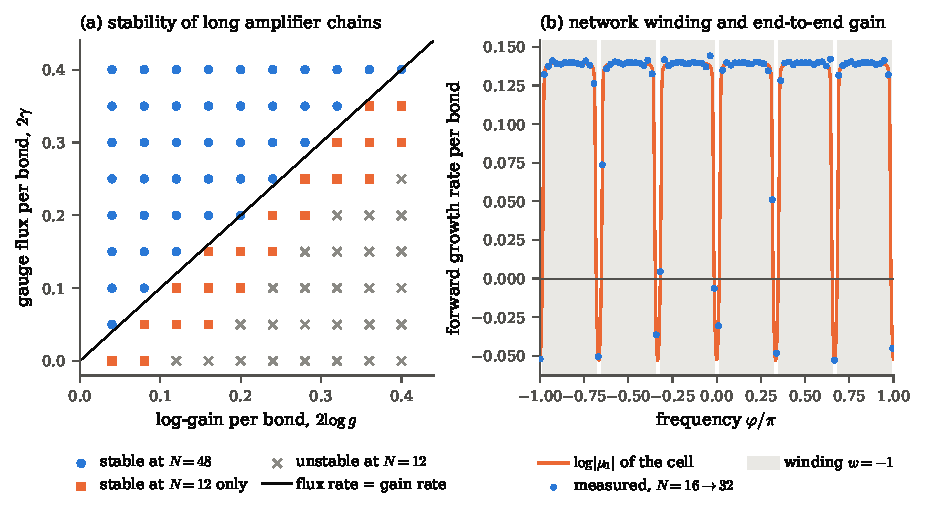
\includegraphics[width=\textwidth]{fig3_lattice.pdf}
\caption{(a) Stability of chains of $N$ bonds, each with a magnitude element of flux $2\gamma$ and an amplifier of log-gain $2\log g$, separated by partial mirrors ($\rho=0.2$). At $N=48$, chains are stable only on or above the diagonal: extensive stable gain requires extensive gauge flux. (b) For $\gamma=0.15$, $g=1.15$: forward growth rate of the end-to-end response, measured between $N=16$ and $N=32$, against $\log|\mu_1|$ of the cell transfer matrix. Shading marks the band where the network winding is $w=-1$.}
\label{fig:lattice}
\end{figure*}

Finally, the flux a cell can supply is bounded. For a passive cell with flat $|S_{21}|=T$ and flux $\lambda$, Theorem~\ref{thm:budget} gives $T(1-e^{-\lambda})\le2\beta$. A magnitude element attains this. A pure-phase element in a Mach--Zehnder cell gives only $\lambda=-\log\cos\frac\Delta2\approx\beta^2/2$, so phase non-reciprocity is a quadratically weaker source of flux. With gain, $\beta$ is replaced by $\sum_i\beta_i(1+\nu_i)$. Combined with Corollary~\ref{cor:rate}, this bounds the log-gain per cell of a robustly stable chain of flat matched cells by $2\,\mathrm{asinh}[\beta_{\rm c}(1+\nu_{\rm c})]$.

%======================================================================
\section{Discussion}\label{sec:disc}

Within this framework the non-Hermitian skin effect is not the resource itself. It is the extensive form of a resource that is conserved in series geometry, the imaginary gauge flux, and what it buys is stable exponential gain (Corollary~\ref{cor:rate}). Skin effects of reciprocal origin carry no such resource and, in quasi-one-dimensional networks, produce neither isolation nor directional amplification (Theorem~\ref{thm:winding}). Loops convert phase-type non-reciprocity into directionality. In passive networks they cannot beat the elementary budget on average; with gain they can, but only at a noise price paid at the non-reciprocal elements.

Several limitations and open problems remain. (i) The results are stated for commensurate delays and frequency-independent devices; a continuum version must account for each device's bandwidth, for instance through gyrotropic sum rules. (ii) $\Cost$ is a faithful monotone, but computing it for dispersive objects is open, and the loop example shows that it can exceed $\NN$ by a factor larger than two. (iii) The optimal efficiency for distilling a perfect broadband isolator from weak elements lies between $1/\pi$ and $1$. (iv) With gain we lack a monotone of the external channel alone. The ring example rules out normalizing $\NN$ by the external excess noise. (v) The correspondence between $w$ and end-to-end rates, and the sharp length-stability threshold for chains with internal reflections, are observed numerically [Fig.~\ref{fig:lattice}] but not proved in general. (vi) Two-dimensional geometry, where reciprocal skin effects live, is outside the present networks. (vii) Time-modulated and parametric devices, in which gain and non-reciprocity come from one element \cite{Kam11,MC15,Mal18}, are non-passive devices; a budget for them needs a noise-aware notion of $\beta$. (viii) The relation between our network-level quantities and the channel-level monotones of Ref.~\cite{MKM26}, which also find a universal unit of time-reversal violation, is open.

%======================================================================
\appendix

\section{Proof of Theorem~\ref{thm:budget}}\label{app:budget}

We may place the external ports on reciprocal junctions, since a reciprocal through-junction and a unit line multiply $S$ by unimodular diagonal factors. Let $P$ embed the device ports into $\mathbb C^I$, and let $\Delta=\bigoplus_iD_{i,A}$. Then $S_J-S_J^\T=2P\Delta P^\T$, $S_{EE}=S_{EE}^\T$ and $S_{EI}^\T=S_{IE}$. From Eq.~\eqref{eq:response} and the push-through identity,
\begin{align*}
S-S^\T&=S_{EI}\bigl[(\one-CS_{II})^{-1}-(\one-CS_{II}^\T)^{-1}\bigr]CS_{IE}\\
&=2X\Delta X^\T,
\end{align*}
with $X=S_{EI}(\one-CS_{II})^{-1}CP$. The second equality follows from the resolvent identity together with $[(\one-CS_{II}^\T)^{-1}CS_{IE}]^\T=X$ on the device ports.

\emph{Energy.} Launch $b_I(0)=Ps$ at $t=0$ with no external input. Because every delay is at least one, nothing arrives at $t=0$. The external output has generating function $X(z)s$. Each launched wave arrives once, attenuated by $|a_\ell|\le1$, so $\sum_{t=1}^T|a_I(t)|^2\le\sum_{t=0}^{T-1}|b_I(t)|^2$. Passivity gives $|y(t)|^2+|b_I(t)|^2\le|a_I(t)|^2$ for $t\ge1$. Summing, $\sum_t|y(t)|^2\le|s|^2$, and Parseval gives $\int|X(re^{i\varphi})s|^2\le|s|^2$ for $r<1$.

\emph{Youla.} Write $D_{i,A}=U_i(\bigoplus_j\sigma_{ij}J)U_i^\T$ with $U_i$ unitary and $J=\left(\begin{smallmatrix}0&1\\-1&0\end{smallmatrix}\right)$ \cite{You61}, so $\Delta=\sum\sigma_{ij}(uw^\T-wu^\T)$ with unit vectors $u,w$ and $\sum_j\sigma_{ij}=\beta(D_i)$. A rank-two skew matrix $M=ab^\T-ba^\T$ has two equal singular values, and $\|M\|_F^2=2(|a|^2|b|^2-|a^\dagger b|^2)$. Hence $\frac12\|M\|_1\le|a||b|$. The triangle inequality, Cauchy--Schwarz and the energy bound give $\int\frac12\|S_A(re^{i\varphi})\|_1\le\sum_i\beta(D_i)$. Fatou's lemma then extends this to the boundary. Direct wiring gives $S=z^2D$.

\section{Proof of Theorem~\ref{thm:noise}}\label{app:noise}

Let $R_k\ge0$ with $R_k\ge S_k^\dagger S_k-\one$. At each junction, $|S_ka|^2\le|a|^2+a^\dagger R_ka$. The energy argument of Appendix~\ref{app:budget} then gives $\sum_t|y(t)|^2\le|s|^2+s^\dagger Es$, where $s^\dagger Es$ is the energy gained by the launched waves. Stability makes all sums finite. Hence $\NN(S)\le\sum_i\beta(D_i)(1+\lambda_{\max}E_i)$.

Now transpose. The network $N^\T$ with junctions $S_k^\T$ and the same lines has response $S^\T$, the same $\NN$, the same budgets, and the same stability, since $\det(\one-S_{II}^\T C)=\det(\one-S_{II}C)$. Apply the bound to $N^\T$ with $R_k=\overline{X_k}$. This is admissible, because $\overline{X_k}\ge0$ and $\overline{X_k}\ge(S_k^\T)^\dagger S_k^\T-\one$. In $N^\T$, the launched waves reach the junction inputs through $(\one-CS_{II}^\T)^{-1}CP=K^\T$, where $K=P^\T(\one-CS_{II})^{-1}C$ carries junction-output noise to the device inputs of $N$. Hence $E_i(N^\T)=\overline{\int K_iXK_i^\dagger}$, whose largest eigenvalue is $\nu_i$. For the equality case, an amplifier $g\sigma_x$ on each port gives $S=g^2z^2D$ and $\nu=g^2-1$.

\section{Proof of Theorem~\ref{thm:winding}}\label{app:winding}

(i) Passivity, $|b_L|^2+|b_R|^2\le|a_L|^2+|a_R|^2$, reads $T^\dagger JT\le J$. On the spectral subspace $V_<$ of eigenvalues inside the disk, $T^nv\to0$ and $(T^nv)^\dagger J(T^nv)\le v^\dagger Jv$, so $V_<$ is $J$-nonnegative. A $J$-nonnegative subspace meets the $m$-dimensional negative subspace only in $0$, so $\dim V_<\le m$. Applying the same argument to $T^{-n}$ on $V_>$ gives $\dim V_>\le m$. (ii) The spectrum is closed under $\mu\mapsto1/\mu$ (Proposition~\ref{prop:series}). (iii) $|\mu_1\mu_2|=|\det T|=1$.

\section{Numerical checks}\label{app:num}

The script \texttt{route2\_nonreciprocity\_toys.py} (numpy and, for the 60-digit lattice computations, mpmath) checks every statement above. Its parts are: A, the golden rule; B, single-frequency non-monotones; C, Theorem~\ref{thm:budget} and the counterexamples to monotonicity of $\NN$; D, the gauge-flux identity and the winding--amplification correspondence; E, the loop principle; F, gain and noise; G, lattices. Each check prints the quantity it tests. The figures are produced by \texttt{paper/make\_figures.py}.

\begin{thebibliography}{99}
\bibitem{Jal13} D. Jalas \emph{et al.}, What is---and what is not---an optical isolator, Nat. Photonics \textbf{7}, 579 (2013).
\bibitem{Cal18} C. Caloz, A. Al\`u, S. Tretyakov, D. Sounas, K. Achouri, and Z.-L. Deck-L\'eger, Electromagnetic nonreciprocity, Phys. Rev. Appl. \textbf{10}, 047001 (2018).
\bibitem{Bar25} S. Barzanjeh, A. Xuereb, A. Al\`u, S. A. Mann, N. Nefedkin, V. Peano, and P. Rabl, Nonreciprocity in quantum technology, arXiv:2508.03945 (2025).
\bibitem{CG19} E. Chitambar and G. Gour, Quantum resource theories, Rev. Mod. Phys. \textbf{91}, 025001 (2019).
\bibitem{BFPW16} K. Bu, H. Fan, A. K. Pati, and J. Wu, Resource theory of special antiunitary asymmetry, arXiv:1610.09646 (2016).
\bibitem{MKM26} J. Miyazaki, K. Kuroiwa, and M. Murao, Dynamical resource theory of time-reversal symmetry breaking, arXiv:2609.36408 (2026).
\bibitem{HN96} N. Hatano and D. R. Nelson, Phys. Rev. Lett. \textbf{77}, 570 (1996).
\bibitem{YW18} S. Yao and Z. Wang, Phys. Rev. Lett. \textbf{121}, 086803 (2018).
\bibitem{KEBB18} F. K. Kunst, E. Edvardsson, J. C. Budich, and E. J. Bergholtz, Phys. Rev. Lett. \textbf{121}, 026808 (2018).
\bibitem{AGU20} Y. Ashida, Z. Gong, and M. Ueda, Adv. Phys. \textbf{69}, 249 (2020).
\bibitem{BBK21} E. J. Bergholtz, J. C. Budich, and F. K. Kunst, Rev. Mod. Phys. \textbf{93}, 015005 (2021).
\bibitem{OKSS20} N. Okuma, K. Kawabata, K. Shiozaki, and M. Sato, Phys. Rev. Lett. \textbf{124}, 086801 (2020).
\bibitem{ZYF20} K. Zhang, Z. Yang, and C. Fang, Phys. Rev. Lett. \textbf{125}, 126402 (2020).
\bibitem{KD19} F. K. Kunst and V. Dwivedi, Non-Hermitian systems and topology: A transfer-matrix perspective, Phys. Rev. B \textbf{99}, 245116 (2019).
\bibitem{Por19} D. Porras and S. Fern\'andez-Lorenzo, Phys. Rev. Lett. \textbf{122}, 143901 (2019).
\bibitem{WBN20} C. C. Wanjura, M. Brunelli, and A. Nunnenkamp, Nat. Commun. \textbf{11}, 3149 (2020).
\bibitem{WBN21} C. C. Wanjura, M. Brunelli, and A. Nunnenkamp, Correspondence between non-Hermitian topology and directional amplification in the presence of disorder, Phys. Rev. Lett. \textbf{127}, 213601 (2021).
\bibitem{ZRR21} H.-G. Zirnstein, G. Refael, and B. Rosenow, Phys. Rev. Lett. \textbf{126}, 216407 (2021).
\bibitem{Xue21} W.-T. Xue, M.-R. Li, Y.-M. Hu, F. Song, and Z. Wang, Simple formulas of directional amplification from non-Bloch band theory, Phys. Rev. B \textbf{103}, L241408 (2021).
\bibitem{BWN23} M. Brunelli, C. C. Wanjura, and A. Nunnenkamp, Restoration of the non-Hermitian bulk-boundary correspondence via topological amplification, SciPost Phys. \textbf{15}, 173 (2023).
\bibitem{MC20} A. McDonald and A. A. Clerk, Nat. Commun. \textbf{11}, 5382 (2020).
\bibitem{Poz12} D. M. Pozar, \emph{Microwave Engineering}, 4th ed. (Wiley, Hoboken, 2012).
\bibitem{Rol62} J. M. Rollett, IRE Trans. Circuit Theory \textbf{9}, 29 (1962).
\bibitem{RA15} L. Ranzani and J. Aumentado, Graph-based analysis of nonreciprocity in coupled-mode systems, New J. Phys. \textbf{17}, 023024 (2015).
\bibitem{MC15} A. Metelmann and A. A. Clerk, Nonreciprocal photon transmission and amplification via reservoir engineering, Phys. Rev. X \textbf{5}, 021025 (2015).
\bibitem{Kam11} A. Kamal, J. Clarke, and M. H. Devoret, Noiseless non-reciprocity in a parametric active device, Nat. Phys. \textbf{7}, 311 (2011).
\bibitem{Mal18} D. Malz, L. D. T\'oth, N. R. Bernier, A. K. Feofanov, T. J. Kippenberg, and A. Nunnenkamp, Quantum-limited directional amplifiers with optomechanics, Phys. Rev. Lett. \textbf{120}, 023601 (2018).
\bibitem{AV73} B. D. O. Anderson and S. Vongpanitlerd, \emph{Network Analysis and Synthesis: A Modern Systems Theory Approach} (Prentice-Hall, Englewood Cliffs, 1973).
\bibitem{MSA19} S. A. Mann, D. L. Sounas, and A. Al\`u, Nonreciprocal cavities and the time--bandwidth limit, Optica \textbf{6}, 104 (2019).
\bibitem{ZYF22} K. Zhang, Z. Yang, and C. Fang, Nat. Commun. \textbf{13}, 2496 (2022).
\bibitem{Wan23} W. Wang, M. Hu, X. Wang, G. Ma, and K. Ding, Experimental realization of geometry-dependent skin effect in a reciprocal two-dimensional lattice, arXiv:2302.06314 (2023).
\bibitem{KSUS19} K. Kawabata, K. Shiozaki, M. Ueda, and M. Sato, Phys. Rev. X \textbf{9}, 041015 (2019).
\bibitem{Gar07} J. B. Garnett, \emph{Bounded Analytic Functions}, revised ed. (Springer, New York, 2007).
\bibitem{Red60} R. Redheffer, J. Math. Phys. \textbf{39}, 269 (1960).
\bibitem{You61} D. C. Youla, Canad. J. Math. \textbf{13}, 694 (1961).
\bibitem{Bi11} L. Bi, J. Hu, P. Jiang, D. H. Kim, G. F. Dionne, L. C. Kimerling, and C. A. Ross, Nat. Photonics \textbf{5}, 758 (2011).
\bibitem{Cav82} C. M. Caves, Phys. Rev. D \textbf{26}, 1817 (1982).
\bibitem{Cle10} A. A. Clerk, M. H. Devoret, S. M. Girvin, F. Marquardt, and R. J. Schoelkopf, Rev. Mod. Phys. \textbf{82}, 1155 (2010).
\end{thebibliography}

\end{document}
